\section{The Energy-Efficient Power Bugeting Method for Multi-Core
  Dark Silicon Systems}

Power budgeting, by the name, provides a power budget which servers
as the maximum allowed/advised system power consumption. For modern multi-core
systems, power consumption is limited by the system heat dissipation
ability. As a result, existing power budgeting methods compute power budget using the maximum
allowed system temperature as the contraint, which enables
high-performance computing for the system. However, the existing power
budgeting methods do not suit for energy-efficient computing
because the temperature dependent leakage power makes the high-performance
(high temperature) state less energy-efficient than some lower-performance
(lower temperature) state. 
In addition, for the dark silicon
multi-core system where not all cores are turned on at the same time,
the system performance and energy-efficiency also depend on the active core distribution, because
different active core distributions lead to different system heat
dissipation abilities.

In this section, we present the energy-efficient power budgeting
method for multi-core dark silicon systems. 
The new method gives a power budget with an optimal/sub-optimal active core distribution which not only maximizes the
energy efficiency (measured as PPW) of the system but also keeps the power budget as high as possible.


% The energy-efficient dynamic power budgeting aims to find the optimal active core distributions and their corresponding DVFS stages, which can maximize the PPW of the multi-core system. While some systems may have constraints other than thermal constraint, such as total power supply limit. But the dark silicon systems are extremely thermal limited, therefore, we focus on the major problem of thermal limits, and other constraints can be added with minor modification if needed.

\subsection{Problem formulation}
PPW is defined as the ratio of the total performance (measured as
instruction per second (IPS)) to the
total power. Because the performance of an active core is linearly
proportional to its clock frequency $f$ as $\ips = \ipc \times f$ where
$\ipc$ stands for instruction per
clock~\cite{Hennessy:Book'12},
we express PPW using clock frequency instead of performance as
\begin{equation}\label{eq:ppw}
\ppw = \frac{\left \| F \right \|_{1}}{\left \| P \right \|_{1}}.
\end{equation}
where $F = [f_1, f_2, \ldots, f_{n_a}]^T$ is a vector containing the
clock frequencies of all active cores (with $f_i$ represents the clock
frequency of the $i$-th active core). 

Then, the energy-efficient power budgeting problem can be formulated as the following optimization problem
\begin{equation}\label{eq:opt_ppw}
\begin{split}
&\text{maximize}~ \ppw = \frac{\left \| F \right \|_{1}}{\left \| P \right \|_{1}}\\
&\text{subject to}  \left\{
\begin{array}{lr}
\card(P) = n_{a},\\
T_{c} \preceq T_{th}.\\
\end{array}
\right.
\end{split}
\end{equation}
where $T_{th} \in \mathbb{R}^{n}$ is the temperature rise threshold
vector containing the maximum allowed temperature rises from the
ambient temperature, $\card(P)$ means the cardinality or size of the vector $P$, which is defined as the number of the nonzero components in $P$. In our case, $\card(P) = n_{a}$ means there are $n_{a}$ active cores.

% Before we solve this optimization problem, in Appendix B, we prove that $\text{PPW}=\frac{\left \| f \right \|_{1}}{\left \| P \right \|_{1}}$ is a quasi-concave function of the clock frequency $f$, which can make sure the optimization problem has a unique solution of $f$ that maximizes PPW.

Solving the optimization problem in \eqref{eq:opt_ppw} directly is
difficult, because power $P$ and clock frequency $F$ are connected by
power model and thermal model (please note that static power is highly
related to temperature) in a complex way as shown previously in
Section~\ref{sec:power_therm_model}. To be specific, the difficulty
comes from two ways. First, the leakage is nonlinear. Second,
temperature of one core is affected by all other cores. 

In order to find the solution in a practical way, we will analyze the PPW
behavior of a single core first, and then consider the temperature coupling
effects to obtain a sub-optimal system PPW as shown in the next part.

% We assume PPW of the system is optimal if the PPW of each core is
% optimal. Therefore, the problem of maximizing the PPW of the system
% can be transformed to maximizing the PPW of each individual core. A
% temperature rise oriented method to obtain sub-optimal PPW of each
% core is shown in next section. 


% The closer $T_{c}$ is to $T_{opt_{n_{a}}}$, the higher the PPW. So instead of
% directly maximizing PPW, the optimization problem in \eqref{eq:opt_ppw} can be transformed to minimizing the difference between $T_{c}$ and $T_{opt_{n_{a}}}$:
% \begin{equation}\label{eq:ppw_minimize_t}
% \begin{split}
% \text{minimize } &  \left \| T_{opt_{n_{a}}}-T_{c} \right \|_{2}\\
% \text{subject to} &\left\{
% \begin{array}{lr}
% \text{card}(P) = n_{a},\\
% T_{c} \preceq T_{th}.\\
% \end{array}
% \right.
% \end{split}
% \end{equation}

% A method to efficiently eliminate the thermal interactions among cores and calculate $T_{opt_{n_{a}}}$ is shown in next section.

\subsection{Energy-efficient power budgeting for a single core}
In this section, we use steady state example to show how to compute
the power budget with the maximum PPW for each core. Please note that
we present the steady state example mainly for the purpose of clarity,
this method is fully functional for transient case. 

% First we prove $T$ is convex w.r.t $f$ in Appendix A, considering for a fixed active core distribution, there is a unique $f$ that can maximize PPW. Therefore, for a fixed active core distribution, there is a unique temperature vector, denoted by $T_{target}$, as long as all cores' temperature rise is the same with the corresponding temperature rise in $T_{target}$, PPW of the system can be maximized. However, $T_{target}$ only works for a fixed active core distribution, the reason is that the thermal interaction among cores varies for different active core distributions. The overhead of obtaining $T_{target}$ for each active core distribution is too high. It is also notices that for a specific core, the optimal temperature rise of it in different active core distributions of the same active core number varies a little. 
% Therefore, for a specific core, we can use a single value to stand for the sub-optimal temperature rise of it in all active core distributions of the same active core number.

% To obtain the sub-optimal temperature rise of each core, we need to isolate the cores. For active core numbers more that $1$, because of the thermal impact active cores have on each other, we need to compensate for the thermal impact of other active cores to correct the error due to isolation of cores.

% An efficient method to isolate the cores and calculate sub-optimal
% temperature rise of each core is proposed in $4.1.1$, and a
% temperature-compensation based method to correctly calculate
% sub-optimal temperature rise for multiply active cores is proposed
% in $4.1.2$.

We first express the PPW of the $i$-th core ($\ppw_i$) in steady state as:
\begin{equation}\label{eq:min_ppw}
\ppw_i=\frac{f_i}{p_{d_i}+p_{s_i}},
\end{equation}
where $p_{d_i}$ and $p_{s_i}$ are the dynamic power and static power
of the $i$-th core, respectively. 

In order to eliminate the nonlinearity in~\eqref{eq:min_ppw}, we
integrate the linearized static power in \eqref{eq:sta_power_lin} into
\eqref{eq:min_ppw} and obtain
\begin{equation}\label{eq:1_ppw}
\ppw_i = \frac{f_i}{p_{d_i}+V_{dd_i}(a_pT_i+I_{0})},
\end{equation}
where $T_i$ is the temperature of the $i$-th core. In \eqref{eq:1_ppw}, there are multiple variables
including $f_i$, $p_{d_i}$, $V_{dd_i}$, and $T_i$. Fortunately, they are all
related to each other in the thermal and power models and thus can be expressed by only one
variable as shown next. Next, we show how to convert all these variables into
$p_{d_i}$, leaving only one variable in~\eqref{eq:1_ppw}.

The major problem of converting all variables into $p_{d_i}$ is that
$T_{i}$ in \eqref{eq:1_ppw} is \emph{not} only influenced by its own
powers $p_{d_i}$ and $p_{s_i}$, but is also affected by powers from
other active cores. As a result, in order to express $T_{i}$ using $p_{d_i}$, we need to
decouple the $i$-th core from the other cores. Please note that the error caused by the
decoupling process can be compensated later. 

Let us first express temperature $T_i$ using $p_{d_i}$. In steady
state, the core temperature vector 
$T_c$ is represented by the power vector $P$ as 
\begin{equation}\label{eq:tc}
T_{c} = B^{T}G^{-1}BP.
\end{equation}
The above formula is obtained by solving the thermal
model~\eqref{eq:therm_model} with the dynamic term $C\frac{dT(t)}{dt}$ ignored
for steady state analysis.
To simplify notification, we let $A = B^{T}G^{-1}B \in \mathbb{R}^{n
  \times n}$, which is defined as the \emph{steady-state thermal
  transfer matrix}~\cite{Reda:SJ'18}.
% Please note that, compared to $G$ matrix, although the size of $A$
% matrix is reduced, all thermal model information including packages
% are reserved.
Then, we can rewrite \eqref{eq:tc} using $A$ matrix as
\begin{equation}\label{eq:sim_tc}
  T_{c} = AP.
\end{equation}
By showing the matrix/vector elements of the above equation, there is
\begin{equation}
{\left[
\begin{matrix}
 T_{1}   \\
 T_{2}   \\
 \vdots  \\
 T_{n}   \\
\end{matrix}
\right]}
=
{\left[
\begin{matrix}
 a_{11} & a_{12} & \cdots & a_{1n} \\
 a_{21} & a_{22} & \cdots & a_{2n} \\
 \vdots & \vdots & \ddots & \vdots \\
 a_{n1} & a_{n2} & \cdots & a_{nn} \\
\end{matrix}
\right]}
{\left[
\begin{matrix}
 p_{1}   \\
 p_{2}   \\
 \vdots  \\
 p_{n}   \\
\end{matrix}
\right]}.\\
\end{equation}
Then, $T_{i}$ can be expressed as
\begin{equation}\label{eq:ti}
T_{i} =a_{i1}p_{1} + a_{i2}p_{2} +\cdots + a_{in}p_{n}. 
\end{equation}

%the diagonal elements $a_{ii}$ in $A$ can be seen as the thermal resistance of core $i$ itself, and the non-diagonal elements $a_{ij}$ in $A$ can be seen as the thermal resistance between core $i$ and $j$. 

In order to express $T_i$ using $p_i$, we \emph{temporally} ignore all
the off-diagonal elements in the $A$ matrix and use only $a_{ii}p_i$ in \eqref{eq:ti} to approximate $T_{i}$ as:
\begin{equation}\label{eq:t_ap}
\begin{split}
T_{i}&\approx a_{ii} \cdot p_{i}\\
&=a_{ii}(p_{d}+p_{s})\\
&=a_{ii}(p_{d}+V_{dd}(p_{0}+a_{s}(T_{i}+T_{amb}))),
\end{split}
\end{equation}
Then, $T_i$ can be readily solved from \eqref{eq:t_ap} as
\begin{equation}\label{eq:ti_new}
T_{i}=\frac{a_{ii}(p_{d}+V_{dd}\cdot p_{0}+V_{dd}\cdot a_{s}\cdot T_{amb})}{1-a_{ii} \cdot a_{s} \cdot V_{dd}}.
\end{equation}

By substituting $T_{i}$ in \eqref{eq:1_ppw} with \eqref{eq:ti_new}, we can have:
\begin{equation}\label{eq:1_ppw_2}
\text{PPW} = \frac{f(1-a_{ii} \cdot a_{s} \cdot V_{dd})}{V_{dd}(a_{s}\cdot T_{amb}+p_{0})+p_{d}},
\end{equation}
which eliminates the thermal impact of other active cores. By substituting $f$ and $V_{dd}$ with $p_{d}$ in \eqref{eq:1_ppw_2}, we can express PPW with only $p_{d}$. The $p_{d}$ that leads to maximum PPW can be obtained with standard gradient search techniques~\cite{Boyd:Convex_BOOK'06}, with which the sub-optimal temperature rise of core $i$ can be calculated from \eqref{eq:ti}.

\begin{figure}
\centering
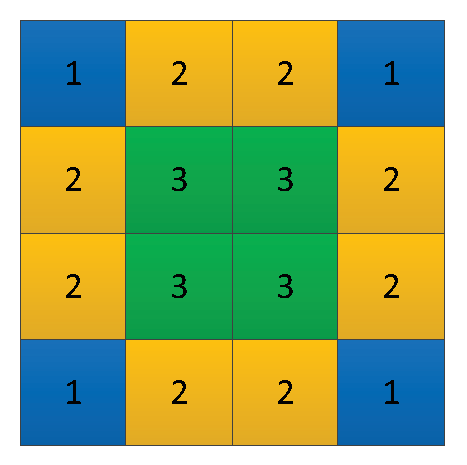
\includegraphics[width=0.46\linewidth]{fig/unique_position.eps}
\caption{$3$ kinds of cores based on their positions in the system for a $16$-core system.}
\label{fig:unique_position}
\end{figure}

Note that we do not need to repeat the calculating process for all cores to obtain all the optimal temperature. All cores can be divided into several kinds based on their position in the system, for a $16$-core system, there are only $3$ kinds of cores which are shown in Fig.~\ref{fig:unique_position}. The cores of the same kind share the same diagonal elements in $A$ matrix. Therefore, calculating the optimal temperature for each kind of core instead of all cores can greatly reduce the computation time.

However, the optimal temperature obtained for isolated cores ignores the thermal impact of other active cores, which is only accurate when there is only $1$ active core. For cases with active cores more than $1$, the thermal interaction among active cores will make the sub-optimal temperature rise deviate from the one we obtained from \eqref{eq:1_ppw_2}. Therefore, a temperature-compensation based method to correctly calculate sub-optimal temperature rise for multiply active cores is introduced in next section.

\begin{table}
  \caption{The energy-efficient power budget induced temperature error for cases with and without $\lambda$. The fixed core is the $1^{st}$ core, for each active core number, $50$ random active core distributions are generated.}
  \label{tab:compensation}
  \centering
  \begin{tabular}{c|c||p{1cm}<{\centering}|p{1cm}<{\centering}||p{1cm}<{\centering}|p{1cm}<{\centering}}
    \hline
    Core & Active     & \multicolumn{2}{c||}{With $\lambda$ ($^{\circ}$C)}  & \multicolumn{2}{c}{Without $\lambda$ ($^{\circ}$C)}\\
\cline{3-6}
    \#       &   \#       &  Avg    & Max &  Avg  &  Max  \\
     \hline
\hline
  \multirow{3}{*}{9} &      2       &   1.1  &   1.9 &2.1&4.0\\
             &      4       &    1.3    &   2.7  &7.0&11.7 \\
             &      7       &   1.2     &   2.2   &13.7&16.1\\
     \hline
   \multirow{3}{*}{16} &      3        &   0.3 &   0.7   &1.5 &2.2 \\   
             &      8       &    0.5     &  1.2  &7.2 &8.3   \\
             &      13     &     0.4    &   1.2  &12.9 &13.7 \\
     \hline
  \multirow{3}{*}{25} &      5       &    0.4 & 1.1 & 3.2 &  4.2   \\ 
              &     12      &    0.5     &    1.4   &  8.7 & 9.9 \\
              &     20      &    0.4     &    1.1   & 13.5 & 14.1 \\ 
     \hline
  \multirow{3}{*}{36}  &     8        &    0.4  &    1.1 & 4.1 & 5.6\\
              &     18      &   0.5      &   1.6  & 10.0 & 11.4  \\
              &     28      &    0.4     &   0.9 & 14.4 & 15.2\\
     \hline
  \multirow{3}{*}{64}  &     12      &   0.4  &   1.2  & 3.8 &4.9 \\
              &     32      &    0.5     &     1.6   & 9.6 & 10.6   \\
              &     52      &     0.4   &     1.0   & 15.9 & 16.5\\
 \hline 
\multirow{3}{*}{100}  & 16 & 	 0.5&	1.1& 3.3 &  4.3\\
                      & 52 &	 0.7&	1.7& 11.4 & 13.0\\
                      & 76 &	 0.5&	1.8& 16.6 & 17.6\\
\hline
\end{tabular}
\end{table}


\subsection{Calculating sub-optimal temperature rise with temperature compensation}
The sub-optimal temperature rise calculated in previous section does not consider of other cores' thermal impact, which could cause major error in dark silicon system, where the temperature rise caused by other cores could make up of a considerable part of the whole temperature rise. Therefore, a compensation method to modify the isolated core's temperature rise $T_{i}$ is proposed in this section.

% \begin{equation}\label{eq:c_full_1_ppw}
% \text{PPW}=\frac{f}{p_{d}+V_{dd}(a_{s}((1+\lambda)T_{i}+T_{a})+p_{0})}.
% \end{equation}
\begin{equation}\label{eq:t_compensation}
\begin{split}
T_{i} &=a_{i1}p_{1} + a_{i2}p_{2} +\cdots + a_{in}p_{n},\\
&\approx(1+\lambda)a_{ii}p_{i}.
\end{split}
\end{equation}

The basic idea of this method is to compensate for the temperature rise caused by other active cores in \eqref{eq:1_ppw} with a parameter $\lambda$, which stands for the temperature rise ratio induced by other active cores, as shown in \eqref{eq:t_compensation}. With $\lambda$, the thermal impact other active cores have on the isolated core can be introduced, therefore the error induced by isolation can be corrected.

The temperature compensation can be perfectly accurate, if for fixed active core distribution, for core $i$ we obtain a $\lambda$, which is calculated as:
\begin{equation}\label{eq:lambda_accuracy}
\lambda =\frac{\sum_{l=1}^{n}a_{il}p_{l}-a_{ii}p_{i}}{a_{ii}p_{i}},
\end{equation}
then the temperature rise caused by other active cores can be compensated without error. However, the overhead would be too high. We find out if we generate a $\lambda$ for each active core number for each kind of core, and assume the power of every active core are the same, the accuracy and overhead can both be satisfactory.
\begin{equation}\label{eq:lambda}
\lambda =\frac{j \cdot \sum_{l=1}^{n}a_{il}-a_{ii}}{a_{ii}},
\end{equation}




% As shown in Fig.~\ref{fig:tavg}, for core $i$, to obtain its $\lambda$ for $4$ active cores, first we calculate the temperature rise $T_{0}$ with core $i$ being the only active core. Then we generate several random active cores distributions with $4$ active cores, and core $i$ is always included in active cores. Note that the power of all active cores are set to be the same. By comparing the averaged temperature rise $T_{avg}$ of core $i$ in the random distributions with $T_{0}$, $\lambda$ for core $i$ with $4$ active cores can be obtained:
% \begin{equation}\label{eq:lambda}
% \lambda = \frac{T_{avg}-T_{0}}{T_{0}}.
% \end{equation}

By repeating the process, we can generate a matrix $\Lambda$, in which $\lambda_{ij}$ stands for the compensation parameter for core $i$ when the active core number is $j$. We substitute the $T_{i}$ in \eqref{eq:1_ppw} with the compensated temperature in \eqref{eq:t_compensation} and get:
\begin{equation}\label{eq:1_ppw_3}
\begin{split}
\text{PPW} =& (\frac{(1+\lambda)(V_{dd}(a_{s}\cdot T_{amb}+p_{0})+p_{d})}{f(1-a_{ii} \cdot a_{s} \cdot V_{dd})}\\
&-\frac{\lambda(p_{d}+V_{dd}(a_{s}\cdot T_{amb}+p_{0}))}{f})^{-1},
\end{split}
\end{equation}

By solving \eqref{eq:1_ppw_3} for every $\lambda$, the sub-optimal temperature rise matrix $T_{opt}$ can be obtained, in which $T_{ij}$ stands for the sub-optimal temperature rise for core $i$ when the active core number is $j$. We can denote each column of $T_{opt}$ as $T_{opt_{n_{a}}}$, where $n_{a}$ is the active core number. 

In order to test the effectiveness of $\lambda$, for example, we first choose a $9$-core system with $4$ active cores, several active core distributions can be generated with core $i$ always turned on. We can obtain the $\lambda_{i}$ for core $i$ for each active core distribution with \eqref{eq:lambda_accuracy}, which ensures perfect accuracy, therefore the sub-optimal temperature rise calculated in this case can be considered "golden". We also obtain the sub-optimal temperature rise calculated both with $\lambda_{i4}$ and without $\lambda$. By comparing the sub-optimal temperature rise of these $2$ cases with "golden", the effective of $\lambda$ can be verified.

In addition to the case shown above, we tested many other systems with different number of cores and active cores. The results are collected in Table~\ref{tab:compensation}.

% \begin{figure}
%   \centering
%   \subfigure[MIPS = 246.3, MIPS/Watt = 2.6]{
%     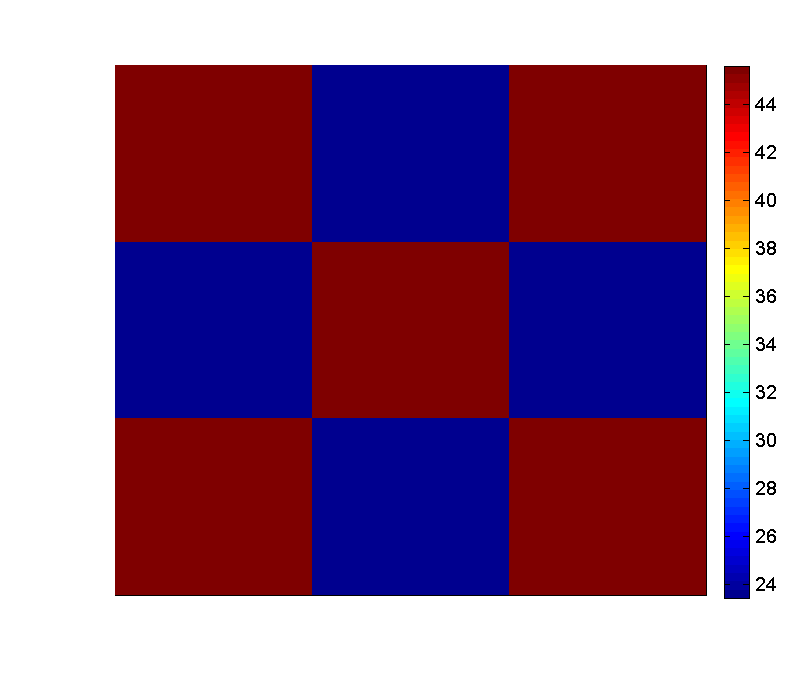
\includegraphics[width=0.46\columnwidth]{fig/opt_tem_1.eps}\label{fig:opt_tem_1}
%   }
%   \hspace{1ex}
%   \subfigure[MIPS = 215.6, MIPS/Watt = 2.6]{
%     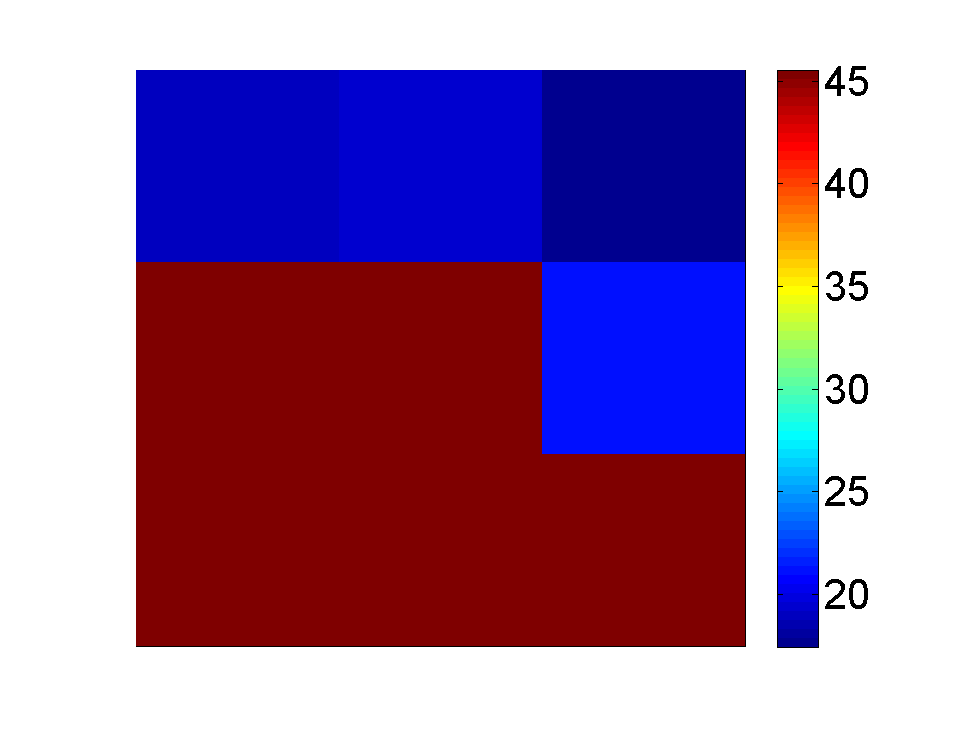
\includegraphics[width=0.46\columnwidth]{fig/opt_tem_2.eps}\label{fig:opt_tem_2}
%   }
%   \caption{Temperature distributions of a 9-core system with 5 cores active in maximum energy efficiency.}
%   \label{fig:opt_tem}
% \end{figure}
\begin{figure}
  \centering
  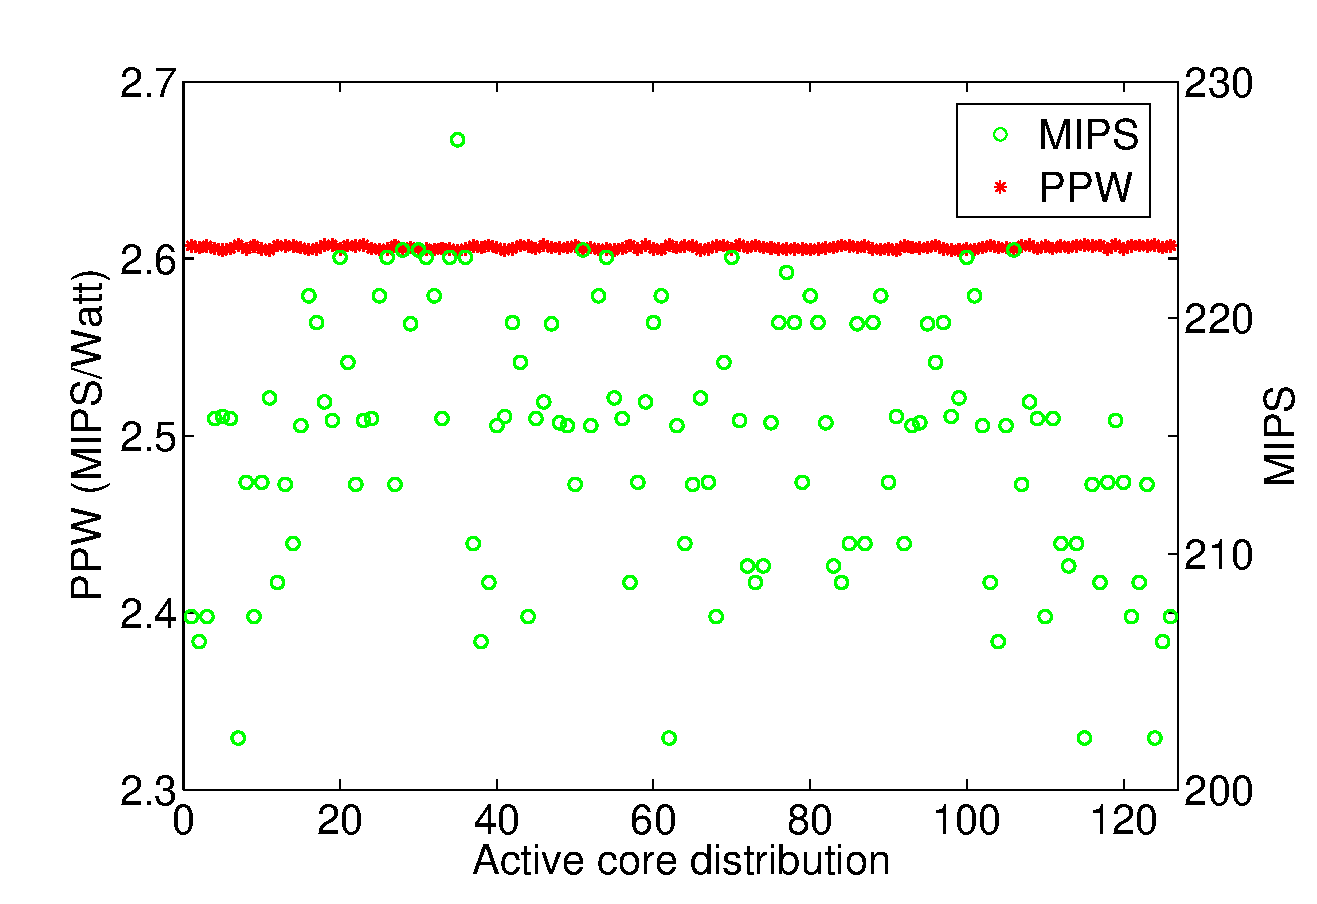
\includegraphics[width=0.9\columnwidth]{fig/mips_ppw.eps}
  \caption{$9$-core system with $4$ active cores. The PPW and MIPS of $126$ possible active core distributions with $T_{opt_{n_{a}}}$ applied are plotted.}
  \label{fig:mips_ppw}
\end{figure}
\begin{figure}
  \centering
  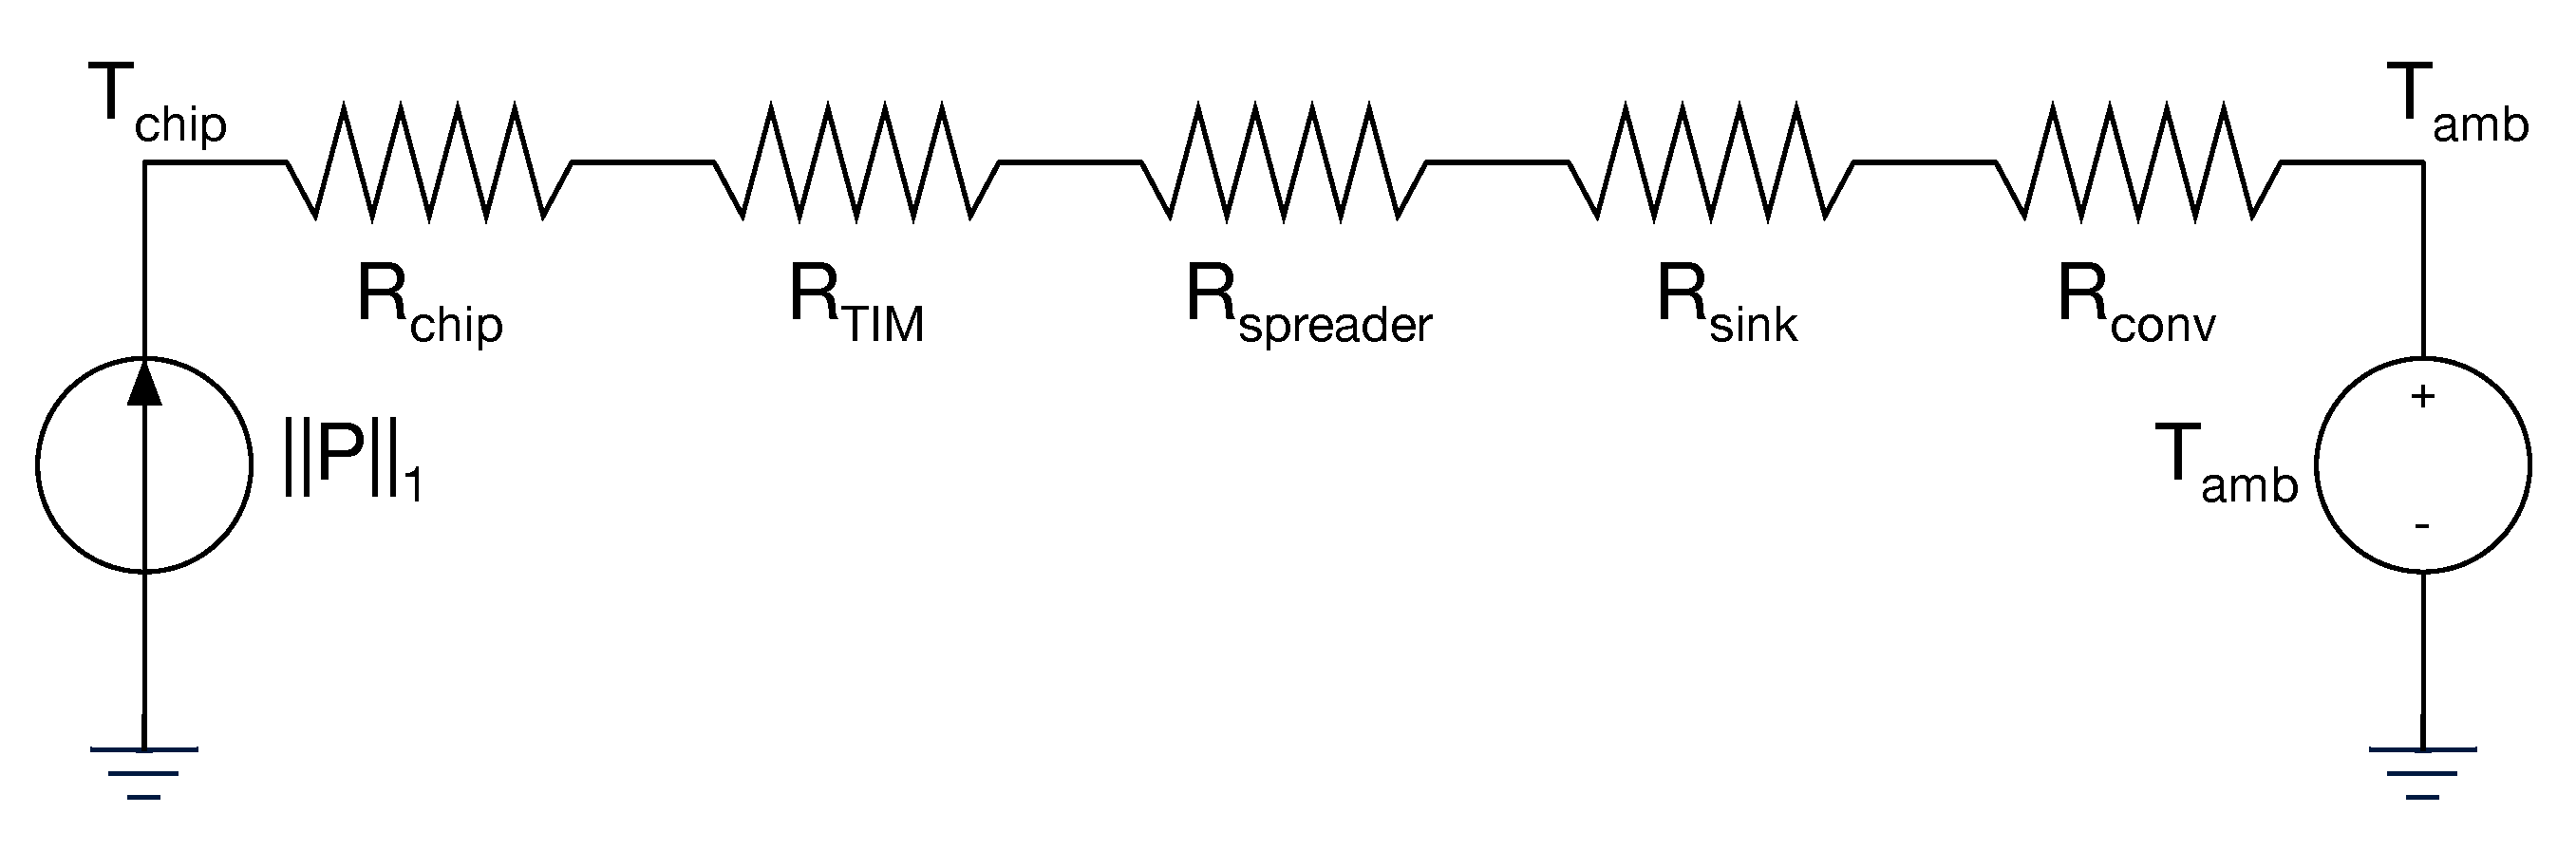
\includegraphics[width=0.8\columnwidth]{fig/resistor_line.eps}
  \caption{The equivalent heat dissipation circuit for normally
    packaged IC chip.}
  \label{fig:resistor_line}
\end{figure}



\subsection{Energy-efficient power budgeting with optimal performance in steady state}
Now that the $T_{opt}$ is obtained, in order to prove $T_{opt_{n_{a}}}$ can leads to sub-optimal PPW of the system for $n_{a}$ active cores, for a $9$-core system with $4$ active cores, we compare the PPW and performance of all active core distributions when $T_{opt_{4}}$ is applied to active cores, which is plotted in Fig.~\ref{fig:mips_ppw}. As can be seen, the PPW of different active core distribution are relatively the same, meaning as long as $T_{opt_{n_{a}}}$ is applied to active cores, the PPW of the system is sub-optimal, no matter what active core distribution it is. However, the performance for different active core distributions differs a lot, which means the performance of the system is affected by the active core distribution greatly in dark silicon system.

Therefore, the goal of our energy-efficient power budgeting is to find the optimal active core distribution that maximizes the power budget, while $T_{opt_{n_{a}}}$ is applied to active cores. Considering it's a combinational problem to find the optimal active core distribution that leads to maximum power budget, in this section, we find out we can formulate an easier alternative problem in which we treat core temperature rise $T_{c}$ as a resource, which is limited by $T_{opt_{n_{a}}}$. In the new problem, we seek to allocate power budget to cores, such that the temperature resource is fully used.

To show the two mentioned problems are equal, we have the following
proposition: 
\begin{proposition}
Providing a normally packaged IC chip, a higher average temperature of
the chip $T_{chip} = \frac{1}{n}\|T_c\|_1 + T_{amb}$ means a higher total power of the
chip $\|P\|_1$, where $T_{amb}$ represents the ambient temperature.
\end{proposition}
\begin{proof}
The proposition above is proved in the following way. The typical structure
of a packaged chip is shown in Fig.~\ref{fig:chip_struct}. Since most heat generated in chip is
conducted through chip, thermal interface material (TIM), heat spreader,
heat sink, and finally dissipated to the air through convection, we
form the equivalent thermal resistor circuit by connecting several
equivalent thermal resistors in series shown in Fig.~\ref{fig:resistor_line}. These thermal resistors represent thermal
resistance in the chip ($R_{chip}$), TIM ($R_{TIM}$), heat spreader
($R_{spreader}$), heat sink ($R_{sink}$), and convection from heat
sink to the air ($R_{conv}$). The two thermal nodes at the two ends of
the thermal circuit denote average temperature of the chip
($T_{chip}=\frac{1}{n}\|T_c\|_1 + T_{amb}$) and average temperature of the
ambient air ($T_{amb}$). 
Because heat is only generated at the chip and only
dissipated into the air, we have an equivalent current source with
current value $\|P\|_1$ (the total power of the chip) connected
at $T_{chip}$ to represent power generation. Also, an equivalent voltage
source is connected at $T_{amb}$ to stand for the ambient air
temperature. Now if we increase the average temperature of the chip,
i.e., increase the value of $T_{chip}=\frac{1}{n}\|T_c\|_1+T_{amb}$, the current flow $\|P\|_1$ in the thermal
resistor circuit has to increase due to the fixed ambient air temperature
$T_{amb}$. In another word, a higher average temperature of
the chip $T_{chip} = \frac{1}{n}\|T_c\|_1 + T_{amb}$ leads to a higher total power of the
chip $\|P\|_1$, which proves the proposition.
\end{proof}

We have shown that higher average temperature of the chip means a higher
total power, and the highest
chip temperature rise limited by the heat dissipation capability is
$T_{th}$, but for temperature higher than $T_{opt_{n_{a}}}$, the energy efficiency will not be maximum. Therefore, the optimization problem of maximizing PPW and optimize power budget can be expressed as:
\begin{equation}\label{eq:sim_opt_topt}
\begin{split}
\text{minimize } &  \left \| T_{opt_{n_{a}}} - AP \right \|_{2}\\
\text{subject to} &\left\{
\begin{array}{lr}
\text{card}(P) = n_{a},\\
AP \preceq T_{opt_{n_{a}}},\\
\end{array}
\right.
\end{split}
\end{equation}
where $AP$ stands for $T_{c}$ from \eqref{eq:sim_tc}.


Finding the optimal solution of such optimization problem requires brute force search of all possible combinations of non-zero positions in $P$ which satisfies $\text{card}(P)=n_{a}$. The high complexity of this method makes it not suitable for multi-core system with large number of cores. It is also noticed that for such systems, finding the optimal solution is not necessary. This is due to the fact that when core number is large, each core takes relatively small area, so there exist many sub-optimal active core distributions which only have slightly larger objective value (measured by cost function) than that of the optimal solution. 
%For example, consider a $25$-core system with $13$ cores active. The optimal solution of such system is shown in xx, and one sub-optimal solution is shown in xx. This is also verified in our experiments by comparing the optimal power budget and the sub-optimal power budget, as shown later.

For a $n$-core system with $n_{a}$ active cores, the basic idea of finding such sub-optimal solution is described as follows: we first find the optimal solution for only one active core. Next, we $fix$ the first active core position determined by the first step, and find the optimal solution of two cores, with the second active core position determined. Please note that although we say "optimal" in the second step, such solution is only the optimal solution with the first active core fixed at the position determined by the first step, not the true optimal solution for general two active cores. Similarly, in the $(i+1)$-th step, we look for the optimal solution for $i+1$ active cores with the position of $i$ active cores found in all previous steps remain fixed. By proceeding such strategy for $n_{a}$ steps, we can arrive at a sub-optimal solution for $n_{a}$ active cores.


To demonstrate the greedy based method in details, we give an example of finding the sub-optimal active core distribution for $n_{a}$ active cores and begin with finding solution for one active core. The optimization problem for one active core is
\begin{equation}\label{eq:1_sim_opt_topt}
\begin{split}
\text{minimize } &  \left \| T_{opt_{n_{a}}} - AP \right \|_{2}\\
\text{subject to} &\left\{
\begin{array}{lr}
\text{card}(P) = 1,\\
AP \preceq T_{opt_{n_{a}}}.\\
\end{array}
\right.
\end{split}
\end{equation}

We have to find a way to determine if one core is superior than the other one, measured by the cost function in \eqref{eq:1_sim_opt_topt}. For the first active core, the way to determine it is simply compare the performance of each core when the $T_{opt_{na}}$ is reached, and choose the core with maximum performance.

Then we show the general iterative steps which are used to find the distribution of $n_{a}$ active cores. Assume we have already fixed the position of $i$ active cores. The corresponding $i$ columns of $A$ are collected into
matrix $A_i \in \mathbb{R}^{i \times n}$, and power budget of these $i$
cores are expressed as vector $P_i \in \mathbb{R}^{i \times 1}$. Then,
we can form the following optimization problem to describe the power
budgeting problem with these $i$ active cores:
\begin{equation}\label{eq:temp_ss_i_pb}
  \begin{split}
    &\text{minimize~~} \|T_{opt_{n_{a}}}-A_i P_i\|_2\\
    &\text{subject to~~} A_i P_i\preceq T_{opt_{n_{a}}}.
  \end{split}
\end{equation}
% The power budget $P_i$ is readily solved by changing
% \eqref{eq:temp_ss_i_pb} into the equivalent QP problem as 
% \begin{equation}\label{eq:temp_ss_i_qp}
%   \begin{split}
%     &\text{minimize~~} P_i^TA_i^TA_iP_i-2T_{th}^TA_iP_i + T_{th}^TT_{th}\\
%     &\text{subject to~~}  A_iP_i \preceq T_{th}.
%   \end{split}
% \end{equation}

\begin{figure}[htb]
\centering
\subfigure[Previous temperature is below $T_{opt_{n_{a}}}$.]{
\begin{minipage}{.45\linewidth}
\centering
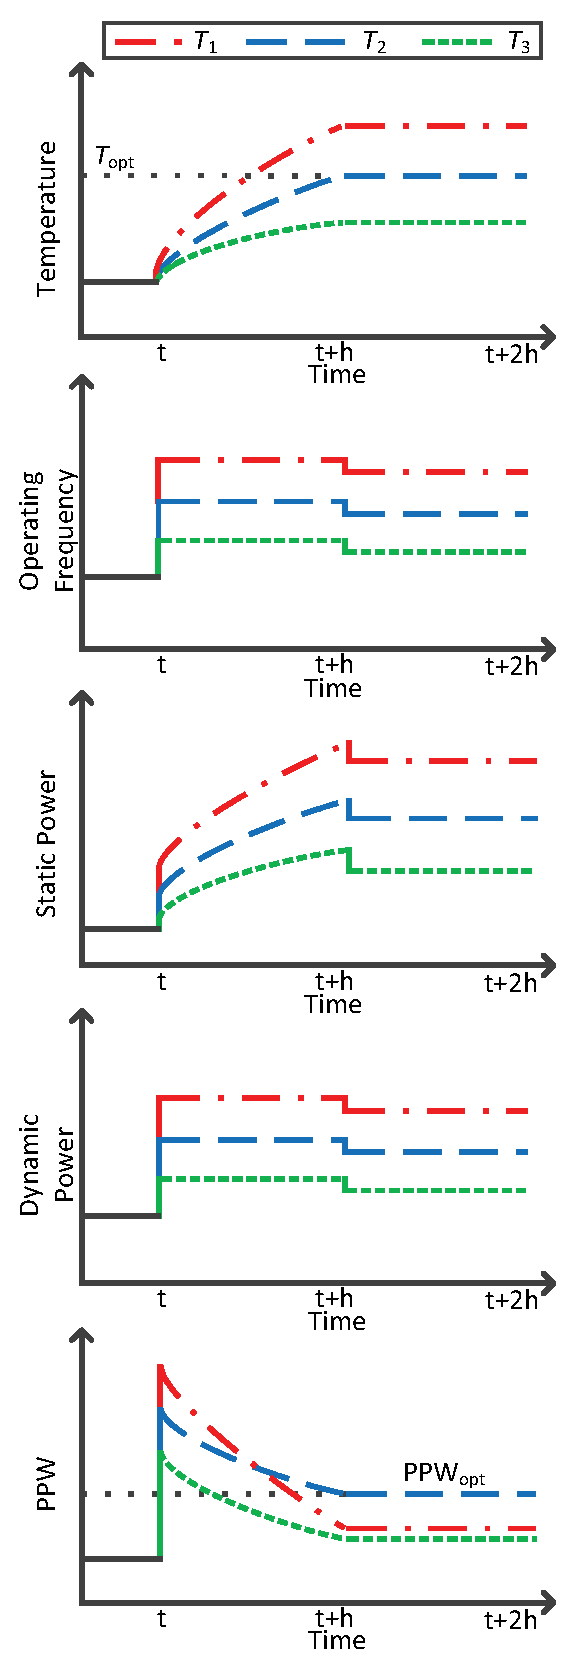
\includegraphics[width=\textwidth]{fig/ppw_boost_1.eps}\label{fig:ppw_boost_1}
\end{minipage}
}
\hfill
\subfigure[Previous temperature is above $T_{opt_{n_{a}}}$.]{
\begin{minipage}{.45\linewidth}
\centering
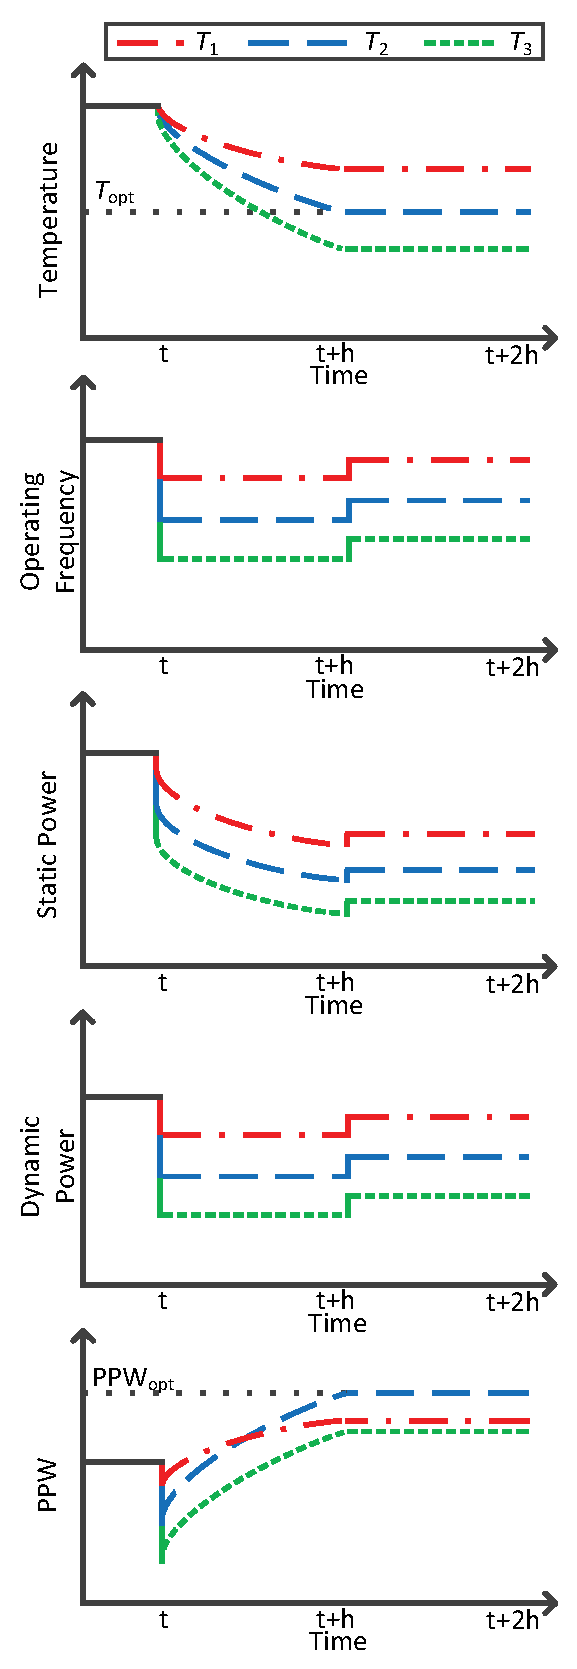
\includegraphics[width=\textwidth]{fig/ppw_boost_2.eps}\label{fig:ppw_boost_2}
\end{minipage}
}
% \subfigure[Previous temperature is $T_{opt_{n_{a}}}$.]{
% \begin{minipage}{.3\linewidth}
% \centering
% 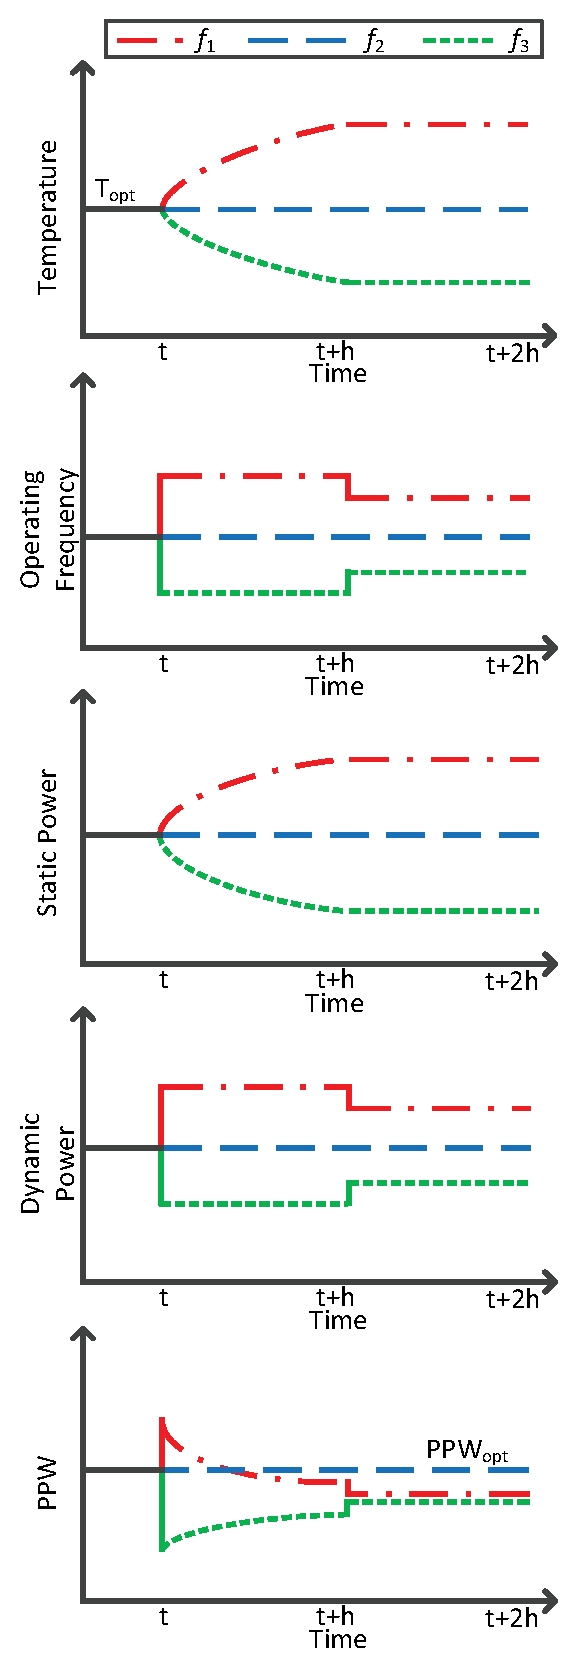
\includegraphics[width=\textwidth]{fig/ppw_boost_3.eps}\label{fig:ppw_boost_3}
% \end{minipage}
% }
\caption{Demonstration of changing temperature and the corresponding PPW. $f_{1}>f_{2}>f_{3}$, and $f_{2}$ can lead to $T_{opt_{n_{a}}}$ in $T(t+h)$.}
\label{fig:ppw_boost}
\end{figure}

In order to find the position of the $(i+1)$-th core, we subtract the temperature rise caused by power budget of $i$ active cores from $T_{opt_{n_{a}}}$, and obtain $T_{rm}=\hat{T}_{opt_{n_{a}}}-A_iP_i$. Next, in order to find which core can complement the impact of the fixed $i$ active cores best, we compare the power budget of each of the rest $n-i$ cores when $T_{rm}$ is reached, and choose the core with maximum power budget.
%One example of comparing two possible active core positions (the $j$-th core and $k$-th core are took as examples) is shown in Fig.x.
%By turning on $j$-th core only, the corresponding temperature rise of the chip is $a_{j}p_{j}$, where $p_{j}$ is the $j$-th elements in $P$ which should be determined by solving \eqref{eq:1_sim_opt_topt}. Assume $p_{j}$ is correctly computed, then the $T_{j}$ component (temperature rise at position $j$) of $a_{j}p_{j}$ should be the same as the $T_{opt_{n_{a}}}$, and $T_{k}$ component of $a_{j}p_{j}$ will be lower than $T_{opt_{n_{a}}}$. Instead, by turning on the $k$-th core only, the corresponding solved power value $p_{k}$ will heat the chip to $a_{k}p_{k}$, with its $T_{j}$ component being lower than $T_{opt_{n_{a}}}$ and its $T_{k}$ component just being equal to $T_{opt_{n_{a}}}$. Between the $j$-th core and $k$-th core, we prefer to turn on the $j$-th core, 


%because its cost $\left \| T_{opt_{n_{a}}}-a_{j}p_{j} \right \|_{2}$ (length of $a_{j}p_{j}-T_{th}$ in xx) in the optimization problem \eqref{eq:1_sim_opt_topt} is smaller than the cost $\left \| T_{opt_{n_{a}}}-a_{k}p_{k} \right \|_{2}$ of turning on the $k$-th core, as observed in Fig. x. The physical meaning is: by turning on the $j$-th core, the overall system temperature is closer to $T_{opt_{n_{a}}}$. With all cores' temperature lower than $T_{opt_{n_{a}}}$, the overall system temperature of turning on the $j$-the core is higher than that of turning on the $k$-th core.




\subsection{Energy-efficient power budgeting with optimal power budget considering transient effects}
The power budgeting method introduced in Section $4.3$ is for steady state condition and serves mostly for illustration of the basic idea of the dynamic power budgeting method. It may work just fine on the aspect of reliability if the computed steady state power budget is followed strictly during the power management process. However, it is frequent that chip switches between high performance mode and high energy efficiency mode, it is also possible that power management makes false decisions occasionally, the computed steady state power budget is not suitable for such scenarios. Therefore, we develop a power budgeting method by considering previous transient thermal/power behaviors as follows.

Before we demonstrate any details, it's necessary to examine the PPW metric in transient state, and prove that the $T_{opt_{n_{a}}}$ obtained in steady state can lead to maximum PPW in transient state.

We focus on a single core $i$, the optimal temperature of it is denoted by $T_{opt_{n_{a}}}(i)$. There are generally $2$ cases in transient state, the previous temperature of the core is below $T_{opt_{i}}$, or above $T_{opt_{i}}$. For each case, based on the target temperature, $3$ scenarios can be classified, which are $T_{1}$, $T_{2}$ and $T_{3}$, where $T_{1}>T_{2}>T_{3}$, and $T_{2} = T_{opt_{n_{a}}}(i)$.

%We assume the clock frequency in one control cycle is fixed, therefore, the $3$ scenarios for each case can be viewed as with different clock frequencies, which are $f_{1}>f_{2}>f_{3}$, and by applying $f_{2}$, $T_{opt_{n_{a}}}$ can be reached in $T(t+h)$, where $h$ is the length of control cycle. We will talk each of the cases in details next.
%in order to improve the PPW of the core, it's necessary to improve the temperature, the difference is how much to improve. We assume the clock frequency in the process is fixed, the goal is to improve the PPW during $t$ and $t+h$, and maintain the temperature of $T_{t+h}$ until $t+2h$. $h$ is the length of control cycle.  Therefore, the $3$ senerios with different frequencies can also be classified by the target temperature by $T(t+h)$. For $f_{1}$, $T(t+h)$ will be higher than $T_{opt_{n_{a}}}$, $f_{2}$ will lead to $T_{opt_{n_{a}}}$ in $t+h$, and for $f_{3}$, $T_{t+h}$ will be lower than $T_{opt_{n_{a}}}$. 

We begin with the case where previous temperature is below $T_{opt_{n_{a}}}(i)$, as Fig.~\ref{fig:ppw_boost_1} shows, for all $3$ scenarios, the target temperature can be reached by the end of the $1^{st}$ control cycle, and in the $2^{nd}$ control cycle, steady state is reached.

Note that there is a sudden drop of frequency in $t+h$ for all target temperatures, which comes from the fact that the power budget provided by our method to increase temperature to target temperature is higher than that of the target temperature in steady state. This means our method can provides "performance boost" when previous temperature is lower than target temperature.

Also as shown in Fig.~\ref{fig:ppw_boost_1}, PPW will increase dramatically in the beginning of the $1^{st}$ control cycle. Especially for target temperature equals to or above $T_{opt_{n_{a}}}(i)$, PPW will temporarily exceed the optimal PPW of steady state, denoted by $\text{PPW}_{opt}$, which means besides "performance boost", our method can also provides "PPW boost". The reason can be obtained from the definition of PPW as
% \begin{equation}\label{eq:ppw_detail}
% \text{PPW} = \frac{\left \| f \right \|_{1}}{\left \| P_{d}+P_{s}(T) \right \|_{1}},
% \end{equation}
\begin{equation}\label{eq:ppw_detail}
\text{PPW} = \frac{f }{p_{d}+p_{s}(T)},
\end{equation}
As shown in Fig.~\ref{fig:ppw_boost_1}, after the instant value change in $t$, $f$and $p_{d}$ will remain constant in the $1^{st}$ control cycle. However, $p_{s}$ is relative to $T$ and $V_{dd}$, as the change of $T$ is not instant, after the instant rise in $t$ caused by $V_{dd}$, $p_{s}$ will slowly rise in the $1^{st}$ control cycle, until the sudden drop in $t+h$ caused by $V_{dd}$. As $p_{s}$ rises in the $1^{st}$ control cycle, PPW first increases to maximum instantly, then declines as $p_{s}$ rises, until to the corresponding value in steady state.

Then we focus on the case where previous temperature is above $T_{opt_{n_{a}}}(i)$, as Fig.~\ref{fig:ppw_boost_2} shows, for all $3$ target temperatures, contrary to the first case, to correct the previous over high temperature, we have to suffer from "performance deterioration" and "PPW deterioration". The "performance deterioration" comes from the fact that in order to reach target temperature by the end of the $1^{st}$ control cycle, the power budget given by our method is lower than that of corresponding target temperature in steady state. The reason of "PPW deterioration" is relatively the same as "PPW boost", which is, as $p_{s}$declines along with $T$ in the $1^{st}$ control cycle, PPW will first decrease to minimum instantly, then increase to the corresponding value in steady state.


% For the last case where previous temperature is $T_{opt_{i}}$, as Fig.~\ref{fig:ppw_boost_3} shows, for $T_{2}$, the power budget is the same as in steady state, therefore, we focus on the other $2$ scenarios. For $T_{1}$, because the target temperature is higher than $T_{opt_{i}}$, there is "PPW boost" in the $1^{st}$ control cycle. For $T_{3}$, it has to suffer from "PPW deterioration" due to lowering temperature.


Next, we focus on verifying the effectiveness of $T_{opt_{n_{a}}}$ in transient state, which equals to proving the overall PPW during a control cycle of $T_{2}$ is the highest among all target temperatures. We can see in Fig.~\ref{fig:ppw_boost}, no matter what previous temperature it is, the PPW of $T_{3}$ is always lower than that of $T_{2}$ in a control cycle. As for $T_{1}$, although the PPW of higher clock frequency will be higher than that of $T_{2}$ in the beginning of the control cycle, the deviation of the target temperature from $T_{opt_{i}}$ makes the PPW of it lower than that of $T_{2}$ in the second half of the control cycle. Overall, the PPW of $T_{1}$ and $T_{2}$ is approximately the same in this control cycle. However, the PPW in the next control cycle is what sets them apart. By remaining the current temperature, the PPW of $T_{1}$ will be lower than that of $T_{2}$. Or, if the temperature is corrected to $T_{opt_{i}}$, the PPW will be even worse because of "PPW deterioration" mentioned above. Therefore, the PPW of applying $T_{2}$ in all circumstances will be maximum among all target temperatures.

With $T_{opt_{n_{a}}}$ being effective in transient state, the basic problem in dynamic power budgeting is to represent temperature rise $T_{c}(t+h)$ using the input power $P$ and initial temperature rise $T_{t}$. Once the formulation of $T_{c}(t+h)$ is available, we can input it into the basic optimization problem \eqref{eq:sim_opt_topt}, and get the sub-optimal $P$ using the similar greedy based method presented in Section $4.2$.

For \eqref{eq:gt}, we can discrete this model using backward Euler's method, and get
\begin{equation}\label{eq:discrete_gt}
(\frac{C}{h}+G)\cdot T(t+h)=\frac{C}{h}T(t)+BP,
\end{equation}
and we are able to express $T_{c}(t+h)$ using $P$ and $T(t)$ as
\begin{equation}\label{eq:discrete_tc}
  \begin{split}
T_{c}(t+h)&=B^{T}T(t+h)\\
&=B^{T}(\frac{C}{h}+G)^{-1}\frac{C}{h}T(t)+B^{T}(\frac{C}{h}+G)^{-1}BP.
  \end{split}
\end{equation}
%\emph{constant}

The cost function of the steady state power budgeting problem in
\eqref{eq:sim_opt_topt} will be changed by using the new $T_c(t+h)$ for
transient case as
\begin{equation}\label{eq:cost_trans}
\|T_{opt_{n_{a}}} -  B^{T}(\frac{C}{h}+G)^{-1}\frac{C}{h}T(t)+B^{T}(\frac{C}{h}+G)^{-1}BP\|_2.
\end{equation}
In order to simplify notation, we denote a new vector  
\begin{equation}
\bar{T}_{opt}=T_{opt_{n_{a}}} - B^{T}(\frac{C}{h}+G)^{-1}\frac{C}{h}T(t),
\end{equation}
where $\bar{T}_{opt}$ has similar meaning of
$T_{opt_{n_{a}}}$ in steady state case, and it also accounts for the transient
thermal effects, i.e., current temperature's impact on power
budget. Also, we denote a new matrix 
\begin{equation}
\bar{A} = B^{T}(\frac{C}{h}+G)^{-1}B, 
\end{equation}
which works similarly as matrix $A$ in steady
state case, but accounts for transient thermal effect. The power
budgeting optimization problem for transient case is updated as 
\begin{equation}\label{eq:temp_ts_opt}
\begin{split}
\text{minimize } &  \left \| \bar{T}_{opt_{n_{a}}}-\bar{A}P \right \|_{2}\\
\text{subject to} &\left\{
\begin{array}{lr}
\text{card}(P) = n_{a},\\
\bar{A}P \preceq \bar{T}_{opt_{n_{a}}}.\\
\end{array}
\right.
\end{split}
\end{equation}
Now dynamic power budgeting can be
applied by following the steps in steady state power budgeting presented in
Section $4.3$, just with \eqref{eq:sim_opt_topt} replaced
by \eqref{eq:temp_ts_opt}.


